\documentclass[a4paper,10pt]{article}

\usepackage[utf8]{inputenc}
\usepackage[english]{babel}
\usepackage[T1]{fontenc}
\usepackage{palatino}

\usepackage[colorlinks=true]{hyperref}
\hypersetup{urlcolor=black,linkcolor=black}

\usepackage{enumerate}

\usepackage{fullpage}
\setlength{\parindent}{0pt}
\setlength{\parskip}{\medskipamount}

\usepackage{amsmath}
\usepackage{amssymb}
\usepackage{mathrsfs}
\usepackage{amsthm}
\usepackage{array}
\usepackage{graphicx}


\title{Project proposal}
\author{PPP \--- ENS Lyon}
\date{M1. 2014}

\begin{document}
\maketitle

\begin{tabular}{|ll|}
\hline
Title & Projet Pensées Profondes (PPP)\\
Coordinator & Marc \textsc{Chevalier}\\
Members & Raphaël \textsc{Charrondière}, Marc \textsc{Chevalier}, Quentin \textsc{Cormier}, \\
        & Tom \textsc{Cornebize}, Yassine \textsc{Hamoudi}, Valentin \textsc{Lorentz},\\
        & Thomas \textsc{Pellissier} \textsc{Tanon}\\
\hline
\end{tabular}

\section{Expected results}
\emph{What is the birth date of the first president of the United States?} This is the typical question that we would like to answer automatically.

This requires three steps. 

Firstly, understanding the natural language. The input string given in standard English has to be transformed into a normal form. To do so, we will use natural language processing (NLP) libraries. We will also implement a machine learning (ML) algorithm, in order to improve the answers of our software.

Then, the normal form is used to collect data, by querying some data base (e.g. Wikidata). Some operations may then be applied, like performing a sort.

Finally, the desired answer is displayed.


\section{Target public}

The first goal of the PPP project is to provide a free, modular and well documented search engine tool that will interest research communities for extensibility features. Our purpose is to allow people to design their own modules and easily include them in the tool. For example, sports modules could be done to answer questions about contests results or upcoming meetings. We intend to make at least one module, using Wikidata, in order to provide a demo and attract the big community of Wikidata.

On the other hand, we also target the potentially users of our tool. We hope to provide a clever, transparent and easy to use search engine tool that will convince people of its utility. At a time when intelligent search engine tools are increasingly used, we think it is now or never for the open source community to propose its own product.

\section{Concurrent services}

Several private companies offer question answering frameworks. 

WolframAlpha \footnote{\url{https://www.wolframalpha.com/}}, a tool developed by 
Wolfram Research, provide a web based service to answer directly to questions asked
in English. It is well known for its abilities to process mathematical statements.
It focuses on historical and scientific facts, such as \emph{When was the French 
revolution?} or \emph{What is the root of pi?}.

Google Now \footnote{\url{http://www.google.com/landing/now/}} and Siri
\footnote{\url{https://www.apple.com/fr/ios/siri/}}, two intelligent personal assistants
developed respectively by Google and Apple, provide a mobile based service to 
answer questions asked in natural language (generally, those of the owner of the
mobile device). They focus on practical facts, such as \emph{Where is the nearest
restaurant?}.

In a first time, the PPP project aims to provide a clever way to browse Wikidata, by giving the 
user the direct answer to his question, not the link of the related Wikipedia
web page. Thus, our software will not be suited to answer such practical questions,
although some new modules can be made if there exists a related database. Google Now
and Siri are therefore not direct concurrent services.

The PPP project is closer to the WolframAlpha tool. However, it is a free project,
and will be modular and well documented. We hope that it will interest the 
Wikipedia community, in order to keep it updated in the future. Moreover,
we will not focus on mathematical questions, as WolframAlpha does.

\section{Software}

The goal is to develop a query answering framework able to answer to simple questions with different back-end. 

\begin{figure}[!h]
    \centering
    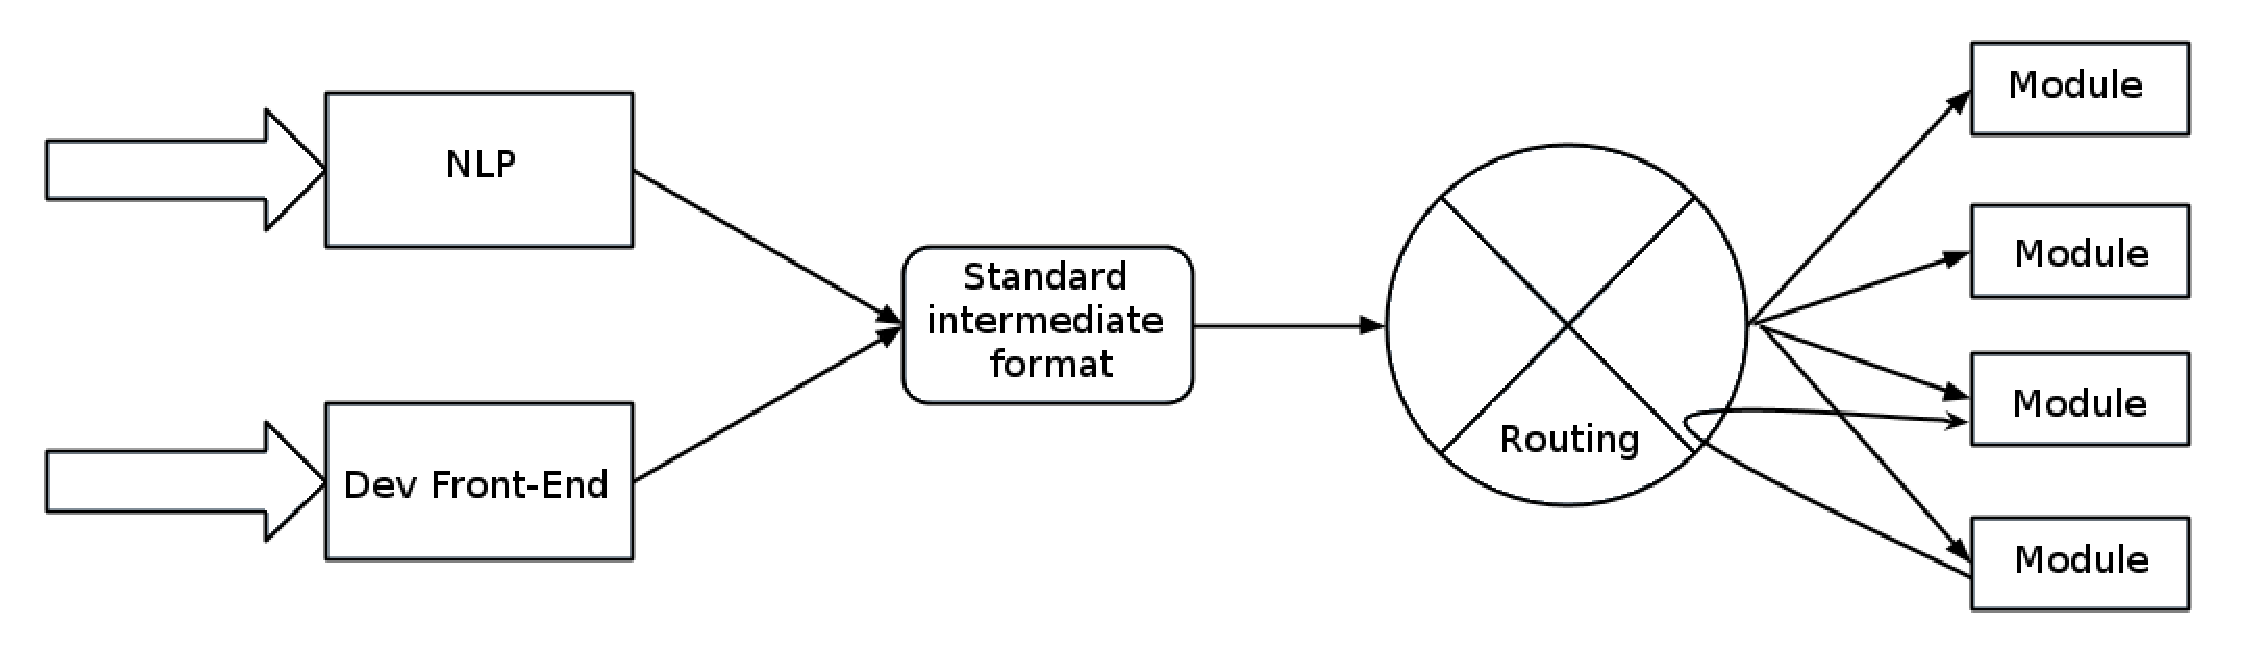
\includegraphics[scale=0.39]{images/Structure-PPP-en.eps}
    \caption{Global structure}
\end{figure}

The software is divided in several components which interact via the HTTP protocol.

First, there are the front-ends which are the user interface. The most natural is a web page, but we can also think about a Android software\ldots Via this interface, we can submit a query.

The query is transformed in a standard form. This form have to be understandable for a computer and describe the question. This work is done in two way. There is a classical natural language processing module and a machine learning-based module. This kind of transformation is very difficult. To avoid having to go through this step, we can develop another front-end for developers which allow to input a question directly in normal form.

The standard form is send into the core. The core's job is routing. It have to send the request in each module to obtain the answers. Sometime, a module can request an answer of another module, for example in the question "what is two times the population of the United States?" which need a geographic data and a mathematical operation. A such question need the successive work of two modules.

To overcome the constraints of language, the core make some request to the Wikidata module to translate each word of the standard for into the associated Wikidata code.

Once a response is generated, it is sent to the interface to be displayed.

A specific module is needed for each database or kind of computation (mathematical, predictive machine learning\ldots).

\section{Technological innovations}


\section{Schedule}

We have planned a simple schedule in two periods.

For the mid-term, we plan to have a functional developer front-end, core, Wikidata module (with the transformation in standard form with Wikidata codes), a first approach of the NLP parser and a base for machine learning.

With this based, the software should be able to answer to simple questions using the developer interface.

For the final term, we plan to have an enhanced NLP parser (especially for the machine learning-based one), a simple web front-end and an enhanced Wikidata module.

Depending on the remaining time, we can develop other modules, e.g. module for OEIS, mathematics\ldots

\section{Task partition}

We decide to form 3 working teams.

A team has to develop the core and the front-ends. It consists of Thomas and Valentin.

Modules are developed by another team made of Thomas, Valentin and Tom. This team should split at the mid-term in a team for enhanced Wikidata module and another team for new modules.

At last, the two NLP parsers are made by the last team made of Yassine, Quentin, Raphaël and Marc.


\section{Organization}

% \section{Budget} not necessary to make a part to explain that there is no budget... just say it in Organization section


\end{document}

